\documentclass[12pt]{article}

\usepackage[utf8]{inputenc}
\usepackage{latexsym,amsfonts,amssymb,amsthm,amsmath}
\usepackage{tikz}
\usepackage{stanli}
\usetikzlibrary{shapes,calc,through,3d}
\usetikzlibrary{decorations.pathreplacing}
\usepackage{multicol}
\usepackage{geometry} 
\usepackage{mathtools}
\usepackage{subcaption}


\setlength{\parindent}{0in}
\setlength{\oddsidemargin}{-0.25in}
\setlength{\textwidth}{7in}
\setlength{\textheight}{9.3in}
\setlength{\topmargin}{-1in}
\setlength{\headheight}{18pt}

\newcommand\blfootnote[1]{%
  \begingroup
  \renewcommand\thefootnote{}\footnote{#1}%
  \addtocounter{footnote}{-1}%
  \endgroup
}

\definecolor{darkred}{rgb}{0.6,0,0}

\newcommand{\bolddelta}{\boldsymbol\delta}


\title{}
\author{Stefano Burzio}
\date{}

\begin{document}

\hrulefill
\vspace{0.3cm}

\hspace*{\fill}\textbf{\Large Archetypal elements and shape functions in 1D}\hspace*{\fill}

\hrulefill

\begin{center}
  \textbf{Linear}
\end{center}
\noindent \newline
\begin{minipage}{0.48\textwidth}
  \begin{tikzpicture}[scale=1.3]
    % Define points
    \coordinate (A) at (-2, 0);
    \coordinate (B) at (2, 0);
    % Mark points
    \fill (A) circle (2pt);
    \fill (B) circle (2pt);
    % Label the element
    \draw[ultra thick] (A) --(B);
    \draw[thick] (-2,-0.5) circle(0.2cm);
    \node at (-2,-0.5) {1};
    \draw[thick] (2,-0.5) circle(0.2cm);
    \node at (2,-0.5) {2};
    \draw[-latex,ultra thin] (-3,0) --(3,0) node[right]{$\xi$};
    \draw[-latex, ultra thin] (0,-0.5) -- (0,2.5);
    \draw[ultra thin] (-.1,2) node[left] {$1$} -- (.1,2);
    %Draw functions 
    \draw[thick, darkred,domain=-2:2, smooth, variable=\x]
    plot ({\x}, {(1-\x/2)});
    \draw[thick, orange,domain=-2:2, smooth, variable=\x]
    plot ({\x}, {(1+\x/2)});
    \node[darkred, above] at (-2, 2) {${}^ah_1(\xi)$};
    \node[orange, above] at (2, 2) {\small ${}^ah_2(\xi)$};
  \end{tikzpicture}
\end{minipage}
\hfill
\begin{minipage}{0.48\textwidth}
  \vfill\centering
  \begin{tabular}{l|l|l}
    Nodes & Coordinates & Base functions            \\ \hline
    1    & $-1$       & ${}^ah_1  =(1-\xi)/2$ \\
    2    & $+1$       & ${}^ah_2  =(1+\xi)/2$ \\
  \end{tabular}
  \vfill
\end{minipage}
\vfill
\begin{center}
  \textbf{Quadratic}
\end{center}
\noindent \newline
\begin{minipage}{0.48\textwidth}
  \begin{tikzpicture}[scale=1.3]
    % Define points
    \coordinate (A) at (-2, 0);
    \coordinate (B) at (2, 0);
    % Mark points
    \fill (A) circle (2pt);
    \fill (B) circle (2pt);
    \fill (0,0) circle (2pt);
    % Label the element
    \draw[ultra thick] (A) --(B);
    \draw[thick] (-2,-0.5) circle(0.2cm);
    \node at (-2,-0.5) {1};
    \draw[thick] (2,-0.5) circle(0.2cm);
    \node at (2,-0.5) {2};
    \draw[thick] (0,-0.5) circle(0.2cm);
    \node at (0,-0.5) {3};
    \draw[-latex,ultra thin] (-3,0) --(3,0) node[right]{$\xi$};
    \draw[-latex, ultra thin] (0,-0.5) -- (0,2.5);
    %Draw functions 
    \draw[thick, orange ,domain=-2:2, smooth, variable=\x]
    plot ({\x}, {\x/2*(\x/2+1)});
    \draw[thick, darkred,domain=-2:2, smooth, variable=\x]
    plot ({\x}, {\x/2*(\x/2-1)});
    \draw[thick, brown,domain=-2:2, smooth, variable=\x]
    plot ({\x}, {2*(1-(\x/2)^2)});
    \node[darkred, above] at (-2, 2) {${}^ah_1(\xi)$};
    \node[orange, above] at (2, 2) {\small ${}^ah_2(\xi)$};
    \node[brown, above right] at (0, 2) {\small ${}^ah_3(\xi)$};
    \draw[ultra thin] (-.1,2) node[left] {$1$} -- (.1,2);
  \end{tikzpicture}\end{minipage}
\hfill
\begin{minipage}{0.48\textwidth}
  \vfill\centering
  \begin{tabular}{l|l|l}
    Nodes & Coordinates & Base functions            \\ \hline
    1    & $-1$       & ${}^ah_1  =\xi(\xi-1)/2$ \\
    2    & $+1$       & ${}^ah_2  =\xi(\xi+1)/2$ \\
    3    & $0$        & ${}^ah_3  =1-\xi^2$      \\
  \end{tabular}
  \vfill
\end{minipage}
\vspace{1cm}
\vfill
\begin{center}
  \textbf{Cubic}
\end{center}
\noindent \newline
\begin{minipage}{0.48\textwidth}
  \begin{tikzpicture}[scale=1.3]
    % Define points
    \coordinate (A) at (-2, 0);
    \coordinate (B) at (2, 0);
    % Mark points
    \fill (A) circle (2pt);
    \fill (B) circle (2pt);
    \fill (-2/3,0) circle (2pt);
    \fill (2/3,0) circle (2pt);
    % Label the element
    \draw[ultra thick] (A) --(B);
    \draw[thick] (-2,-0.5) circle(0.2cm);
    \node at (-2,-0.5) {1};
    \draw[thick] (2,-0.5) circle(0.2cm);
    \node at (2,-0.5) {2};
    \draw[thick] (-2/3,-0.5) circle(0.2cm);
    \node at (-2/3,-0.5) {3};
    \draw[thick] (2/3,-0.5) circle(0.2cm);
    \node at (2/3,-0.5) {4};
    \draw[-latex,ultra thin] (-3,0) --(3,0) node[right]{$\xi$};
    \draw[-latex, ultra thin] (0,-0.5) -- (0,2.5);
    %Draw functions 
    \draw[thick, darkred ,domain=-2:2, smooth, variable=\x]
    plot ({\x}, {-(1-\x/2)*(1-9*(\x/2)^2)/8});
    \draw[thick, orange,domain=-2:2, smooth, variable=\x]
    plot ({\x}, {-(1+\x/2)*(1-9*(\x/2)^2)/8});
    \draw[thick, brown,domain=-2:2, smooth, variable=\x]
    plot ({\x}, {9*(1-3*\x/2)*(1-(\x/2)^2)/8});
    \draw[thick, purple,domain=-2:2, smooth, variable=\x]
    plot ({\x}, {9*(1+3*\x/2)*(1-(\x/2)^2)/8});
    \node[darkred, above] at (-2, 2) {${}^ah_1(\xi)$};
    \node[orange, above] at (2, 2) {\small ${}^ah_2(\xi)$};
    \node[brown, above left] at (0, 2) {\small ${}^ah_3(\xi)$};
    \node[purple, above right] at (0, 2) {\small ${}^ah_4(\xi)$};
    \draw[ultra thin] (-.1,2) node[left] {$1$} -- (.1,2);
  \end{tikzpicture}
\end{minipage}
\hfill
\begin{minipage}{0.48\textwidth}
  \vfill\centering
  \begin{tabular}{l|l|l}
    Nodes & Coordinates & Base functions            \\ \hline
    1    & $-1$       & ${}^ah_1  =-(1-\xi)(1-9\xi^2)/16$ \\
    2    & $+1$       & ${}^ah_2  =-(1+\xi)(1-9\xi^2)/16$ \\
    3    & $-1/3$     & ${}^ah_3  =9(1-3\xi)(1-\xi^2)/16$ \\
    4    & $1/3$      & ${}^ah_4  =9(1+3\xi)(1-\xi^2)/16$ \\
  \end{tabular}
  \vfill
\end{minipage}
\vfill

%%%%%2D
\newpage
\hrulefill
\vspace{0.3cm}

\hspace*{\fill}\textbf{\Large Archetypal elements and shape functions in 2D}\hspace*{\fill}

\hrulefill

\vfill
\begin{center}
  \textbf{Bilinear quadrilateral}
\end{center}\vspace{-1cm}
\noindent \newline
\begin{minipage}{0.38\textwidth}
  \begin{tikzpicture}[scale=1.5]
    \def\a{2}
    \def\b{2}
    \coordinate (x1) at (0, 0);
    \coordinate (x2) at (\a, 0);
    \coordinate (x3) at (0, \b);
    \coordinate (x4) at (\a, \b);
    \filldraw[gray!10] (x1) -- (x2) -- (x4) -- (x3) -- cycle;
    \draw[ultra thick] (x1) -- (x2) -- (x4) -- (x3) -- cycle;
    \draw[fill=white, thick] (x1) node{1} circle(0.2cm);
    \draw[fill=white, thick] (x2) node{2} circle(0.2cm);
    \draw[fill=white, thick] (x3) node{4} circle(0.2cm);
    \draw[fill=white, thick] (x4) node{3} circle(0.2cm);
    \draw[-latex,ultra thin] (-1,\b/2) -- (\a+1,\b/2) node[right]{$\xi_1$};
    \draw[-latex,ultra thin] (\a/2,-1) -- (\a/2,\b+1) node[above]{$\xi_2$};
  \end{tikzpicture}
\end{minipage}
\hfill
\begin{minipage}{0.58\textwidth}
  \vfill\centering
  \begin{tabular}{l|l|l}
    Nodes & Coordinates & Base functions            \\ \hline
    1    & $(-1,-1)$   & ${}^ah_1   = (1-\xi_1)(1-\xi_2)/4 $ \\
    2    & $(+1,-1)$   & $ {}^ah_2  = (1+\xi_1)(1-\xi_2)/4 $ \\
    3    & $(+1,+1)$   & $ {}^ah_3  = (1+\xi_1)(1+\xi_2)/4 $ \\
    4    & $(-1,+1)$   & $ {}^ah_4  = (1-\xi_1)(1+\xi_2)/4$  \\
  \end{tabular}
  \vfill
\end{minipage}
\vfill
\begin{center}
  \textbf{Biquadratic quadrilateral}
\end{center}\vspace{-0.5cm}
\noindent \newline
\begin{minipage}{0.38\textwidth}
  \begin{tikzpicture}[scale=1.5]
    \def\a{2}
    \def\b{2}
    \coordinate (x1) at (0, 0);
    \coordinate (x2) at (\a, 0);
    \coordinate (x3) at (0, \b);
    \coordinate (x4) at (\a, \b);
    \coordinate (x5) at (\a/2, 0);
    \coordinate (x6) at (\a, \b/2);
    \coordinate (x7) at (\a/2, \b);
    \coordinate (x8) at (0, \b/2);
    \coordinate (x9) at (\a/2, \b/2);
    \filldraw[gray!10] (x1) -- (x2) -- (x4) -- (x3) -- cycle;
    \draw[ultra thick] (x1) -- (x2) -- (x4) -- (x3) -- cycle;
    \draw[-latex,ultra thin] (-1,\b/2) -- (\a+1,\b/2) node[right]{$\xi_1$};
    \draw[-latex,ultra thin] (\a/2,-1) -- (\a/2,\b+1) node[above]{$\xi_2$};
    \draw[fill=white, thick] (x1) node{1} circle(0.2cm);
    \draw[fill=white, thick] (x2) node{2} circle(0.2cm);
    \draw[fill=white, thick] (x3) node{4} circle(0.2cm);
    \draw[fill=white, thick] (x4) node{3} circle(0.2cm);
    \draw[fill=white, thick] (x5) node{5} circle(0.2cm);
    \draw[fill=white, thick] (x6) node{6} circle(0.2cm);
    \draw[fill=white, thick] (x7) node{7} circle(0.2cm);
    \draw[fill=white, thick] (x8) node{8} circle(0.2cm);
    \draw[fill=white, thick] (x9) node{9} circle(0.2cm);
  \end{tikzpicture}
\end{minipage}
\hfill
\begin{minipage}{0.58\textwidth}
  \vfill\centering
  \begin{tabular}{l|l|l}
    Nodes & Coordinates & Base functions            \\ \hline
    1    & $(-1,-1)$   & $ {}^ah_1  = \xi_1\xi_2(\xi_1-1)(\xi_2-1)/4$  \\
    2    & $(1,-1)$    & ${}^ah_2= \xi_1\xi_2(\xi_1+1)(\xi_2-1)/4$     \\
    3    & $(1,1)$     & $ {}^ah_3  = \xi_1\xi_2(\xi_1+1)(\xi_2+1)/4 $ \\
    4    & $(-1,1)$    & $ {}^ah_4 = \xi_1\xi_2(\xi_1-1)(\xi_2+1)/4$   \\
    5    & $(0,-1)$    & $ {}^ah_5  = \xi_2(1-\xi_1^2)(\xi_2-1)/2 $    \\
    6    & $(1,0)$     & $ {}^ah_6  = \xi_1(\xi_1+1)(1-\xi_2^2)/2   $  \\
    7    & $(0,1)$     & $ {}^ah_7  = \xi_2(1-\xi_1^2)(\xi_2+1)/2   $  \\
    8    & $(-1,0)$    & $ {}^ah_8  = \xi_1(\xi_1-1)(1-\xi_2^2)/2  $   \\
    9    & $(0,0)$     & $ {}^ah_9  = (1-\xi_1^2)(1-\xi_2^2)/2  $      \\
  \end{tabular}
  \vfill
\end{minipage}
\vfill

\newpage
\vfill
\begin{center}
  \textbf{Bilinear triangular}
\end{center}\vspace{-1cm}
\noindent \newline
\begin{minipage}{0.38\textwidth}
  \begin{tikzpicture}[scale=1.5]
    \def\a{2}
    \def\b{2}
    \coordinate (x1) at (0, 0);
    \coordinate (x2) at (\a, 0);
    \coordinate (x3) at (0, \b);
    \filldraw[gray!10] (x1) -- (x2) -- (x3) -- cycle;
    \draw[ultra thick] (x1) -- (x2)-- (x3) -- cycle;
    \draw[-latex,ultra thin] (-1,0) -- (\a+1,0) node[right]{$\xi_1$};
    \draw[-latex,ultra thin] (0,-1) -- (0,\b+1) node[above]{$\xi_2$};
    \draw[fill=white, thick] (x1) node{1} circle(0.2cm);
    \draw[fill=white, thick] (x2) node{2} circle(0.2cm);
    \draw[fill=white, thick] (x3) node{3} circle(0.2cm);
  \end{tikzpicture}
\end{minipage}
\hfill
\begin{minipage}{0.58\textwidth}
  \vfill\centering
  \begin{tabular}{l|l|l}
    Nodes & Coordinates & Base functions            \\ \hline
    1    & $(0,0)$     & ${}^ah_1  = 1-\xi_1-\xi_2$ \\
    2    & $(1,0)$     & $  {}^ah_2  = \xi_1 $      \\
    3    & $(0,1)$     & $ {}^ah_3  = \xi_2      $  \\
  \end{tabular}
  \vfill
\end{minipage}
\vfill
\begin{center}
  \textbf{Biquadratic triangular}
\end{center}\vspace{-1cm}
\noindent \newline
\begin{minipage}{0.38\textwidth}
  \begin{tikzpicture}[scale=1.5]
    \def\a{2}
    \def\b{2}
    \coordinate (x1) at (0, 0);
    \coordinate (x2) at (\a, 0);
    \coordinate (x3) at (0, \b);
    \coordinate (x4) at (\a/2,0);
    \coordinate (x5) at (\a/2, \b/2);
    \coordinate (x6) at (0, \b/2);
    \filldraw[gray!10] (x1) -- (x2) -- (x3) -- cycle;
    \draw[ultra thick] (x1) -- (x2)-- (x3) -- cycle;
    \draw[-latex,ultra thin] (-1,0) -- (\a+1,0) node[right]{$\xi_1$};
    \draw[-latex,ultra thin] (0,-1) -- (0,\b+1) node[above]{$\xi_2$};
    \draw[fill=white, thick] (x1) node{1} circle(0.2cm);
    \draw[fill=white, thick] (x2) node{2} circle(0.2cm);
    \draw[fill=white, thick] (x3) node{3} circle(0.2cm);
    \draw[fill=white, thick] (x4) node{4} circle(0.2cm);
    \draw[fill=white, thick] (x5) node{5} circle(0.2cm);
    \draw[fill=white, thick] (x6) node{6} circle(0.2cm);
  \end{tikzpicture}
\end{minipage}
\hfill
\begin{minipage}{0.58\textwidth}
  \vfill\centering
  \begin{tabular}{l|l|l}
    Nodes & Coordinates & Base functions            \\ \hline
    1    & $(0,0)$     & ${}^ah_1  = (1-\xi_1-\xi_2)(1-2\xi_1-2\xi_2)$ \\
    2    & $(1,0)$     & $  {}^ah_2  = \xi_1(2\xi_1-1) $               \\
    3    & $(0,1)$     & $ {}^ah_3  = \xi_2(2\xi_2-1)      $           \\
    4    & $(1/2,0)$   & $ {}^ah_4 = 4\xi_1(1-\xi_1-\xi_2)       $     \\
    5    & $(1/2,1/2)$ & $ {}^ah_5  = 4\xi_1\xi_2      $               \\
    6    & $(0,1/2)$   & $ {}^ah_6 = 4\xi_2(1-\xi_1-\xi_2)      $      \\
  \end{tabular}
  \vfill
\end{minipage}
\vfill




\end{document}